\chapter{Diagramas Esquem�ticos}
\label{ap:HWSch}

\begin{figure}[htb]
\begin{center}
 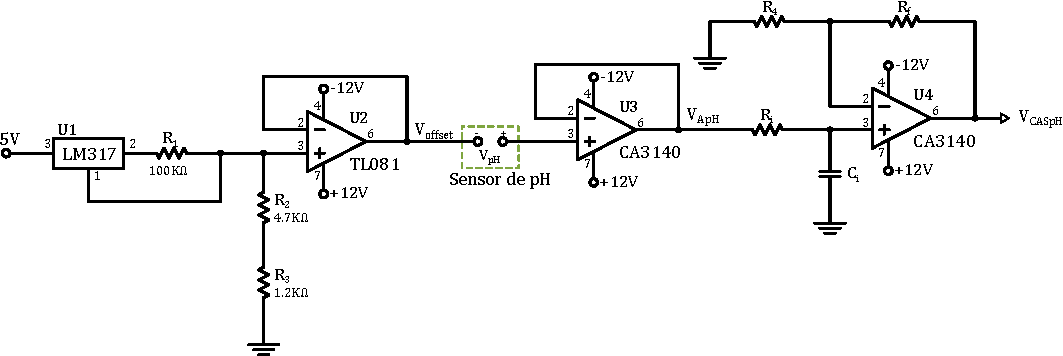
\includegraphics[scale=0.9]{Imagenes/Desarrollo/Dise�oHardware/CASpH_full.pdf}
\end{center}
 \caption{Diagrama esquem�tico del dispositivo CAS para el sensor de pH.} \label{fig:ap:CASpH_full}
\end{figure}

\begin{figure}[htb]
\begin{center}
 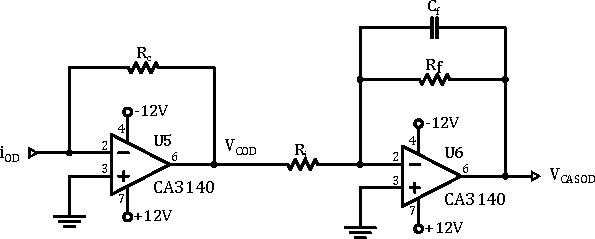
\includegraphics[scale=0.9]{Imagenes/Desarrollo/Dise�oHardware/CASOD_full.pdf}
\end{center}
 \caption{Diagrama esquem�tico del dispositivo CAS para el sensor de OD.} \label{fig:ap:CASOD_full}
\end{figure}

\begin{figure}[htb]
\begin{center}
 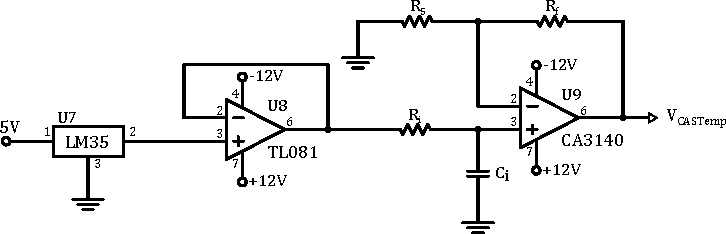
\includegraphics[scale=0.9]{Imagenes/Desarrollo/Dise�oHardware/CASTemp.pdf}
\end{center}
 \caption{Diagrama esquem�tico del dispositivo CAS para el sensor de temperatura.} \label{fig:ap:CASTemp}
\end{figure}

\begin{figure}[htb]
\begin{center}
 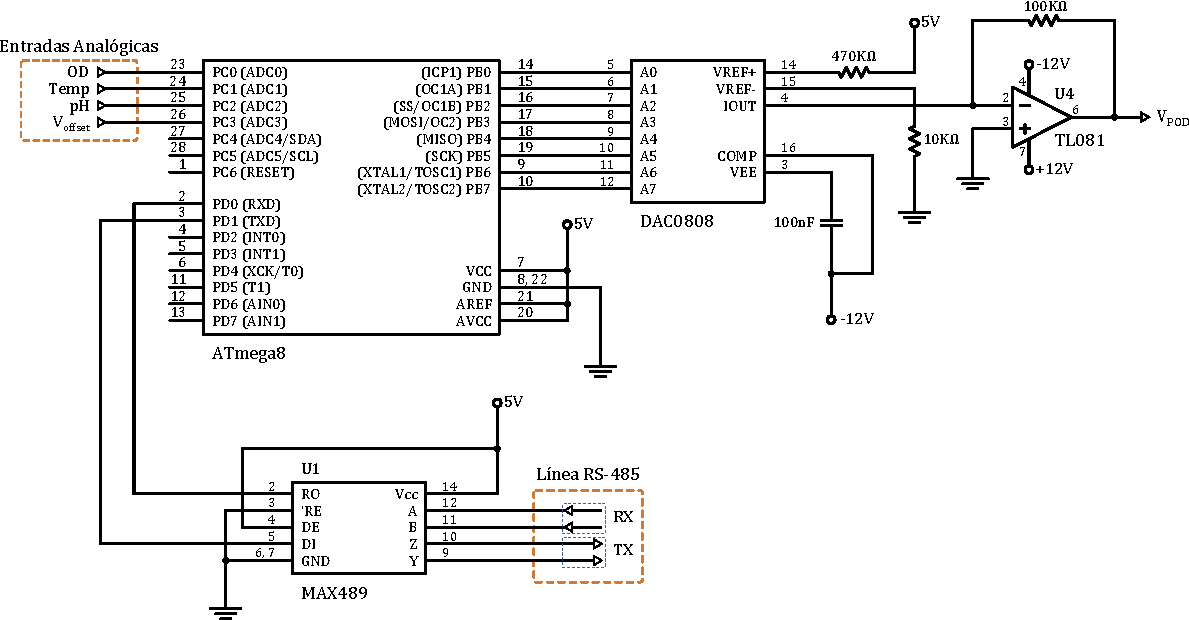
\includegraphics[scale=0.85]{Imagenes/Desarrollo/Dise�oHardware/MCU_schematic.pdf}
\end{center}
 \caption{Diagrama esquem�tico para las entradas y salidas del MCU.} \label{fig:ap:MCU_schematic}
\end{figure}

\chapter{PCB}
\label{ap:PCB}

\begin{figure}[htb]
	\begin{center}
		\begin{tabular}{c}
			\subfloat[Dise�o de pistas PCB de capa inferior.]{%
				\label{fig:ap:RTUMTU2}%
				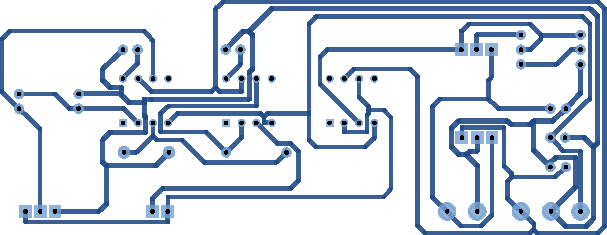
\includegraphics[scale=1]{Imagenes/Desarrollo/Integracion/CASpH.pdf}} \\
			\subfloat[Ordenamiento de CIs.]{%
				\label{fig:ap:MTU-Servidores}%
				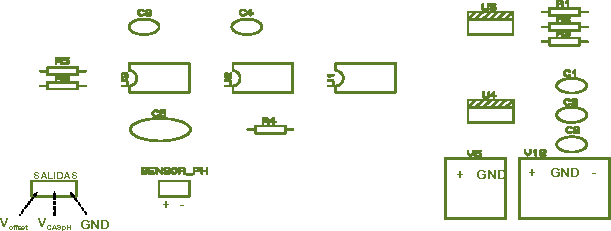
\includegraphics[scale=1]{Imagenes/Desarrollo/Integracion/CASpHCIs.pdf}} \\
		\end{tabular}
	\end{center}
	\caption{PCB del CAS para el sensor de pH.} \label{fig:ap:PCBCASpH}
\end{figure}

\begin{figure}[htb]
	\begin{center}
		\begin{tabular}{c}
			\subfloat[Dise�o de pistas PCB de capa inferior.]{%
				\label{fig:ap:RTUMTU2}%
				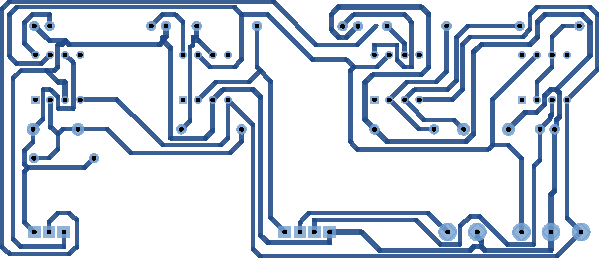
\includegraphics[scale=1]{Imagenes/Desarrollo/Integracion/CASODTemp.pdf}} \\
			\subfloat[Distribuci�n de CIs.]{%
				\label{fig:ap:MTU-Servidores}%
				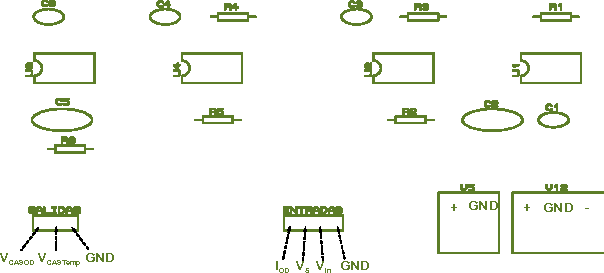
\includegraphics[scale=1]{Imagenes/Desarrollo/Integracion/CASODTempCIs.pdf}} \\
		\end{tabular}
	\end{center}
	\caption{PCB del CAS para el sensor de OD y temperatura.} \label{fig:ap:PCBCASODTemp}
\end{figure}

\begin{figure}[htb]
	\begin{center}
		\begin{tabular}{c}
			\subfloat[Dise�o de pistas PCB de capa inferior.]{%
				\label{fig:ap:RTUMTU2}%
				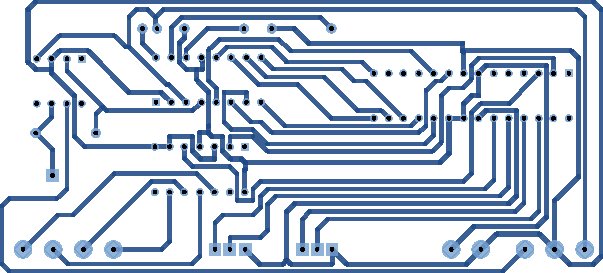
\includegraphics[scale=1]{Imagenes/Desarrollo/Integracion/MCU.pdf}} \\
			\subfloat[Distribuci�n de CIs.]{%
				\label{fig:ap:MTU-Servidores}%
				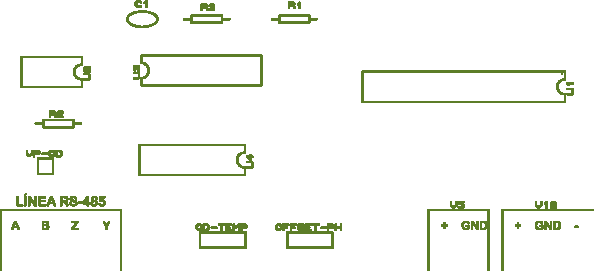
\includegraphics[scale=1]{Imagenes/Desarrollo/Integracion/MCUCIs.pdf}} \\
		\end{tabular}
	\end{center}
	\caption{PCB para el m�dulo del MCU.} \label{fig:ap:MCUPCB}
\end{figure}

\begin{figure}[htb]
	\begin{center}
		\begin{tabular}{cc}
			\subfloat[Dise�o de pistas PCB de capa inferior.]{%
				\label{fig:ap:RTUMTU2}%
				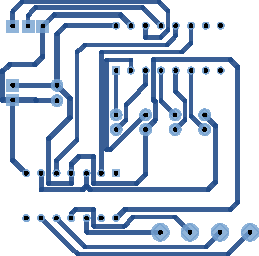
\includegraphics[scale=0.9]{Imagenes/Desarrollo/Integracion/RS232-RS485.pdf}} &
			\subfloat[Distribuci�n de CIs.]{%
				\label{fig:ap:MTU-Servidores}%
				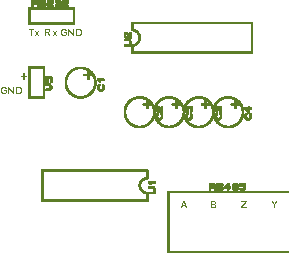
\includegraphics[scale=0.9]{Imagenes/Desarrollo/Integracion/RS232-RS485CIs.pdf}} \\
		\end{tabular}
	\end{center}
	\caption{PCB del transceptor RS-232/RS-485.} \label{fig:ap:RS232-RS485PCB}
\end{figure}

\chapter{Dise�o Software}
\label{ap:SWMTU}

\section{Clases}
\label{ap:SWMTU:Class}

Para una mejor comprensi�n de la divisi�n de subprocesos del software de la MTU (Secci�n~\ref{cap3:DSWMTU}) los diagramas de clase se dividen en cinco secciones: monitoreo de entradas anal�gicas (Figura~\ref{fig:ap:MTUClassEA}), monitoreo de entradas digitales (Figura~\ref{fig:ap:MTUClassED}), diagrama de monitoreo y control de salidas digitales (Figura~\ref{fig:ap:MTUClassSD}) y calibraci�n de sensores (Figura~\ref{fig:ap:MTUClassCalibracion}).

\begin{figure}[H]
\begin{center}
 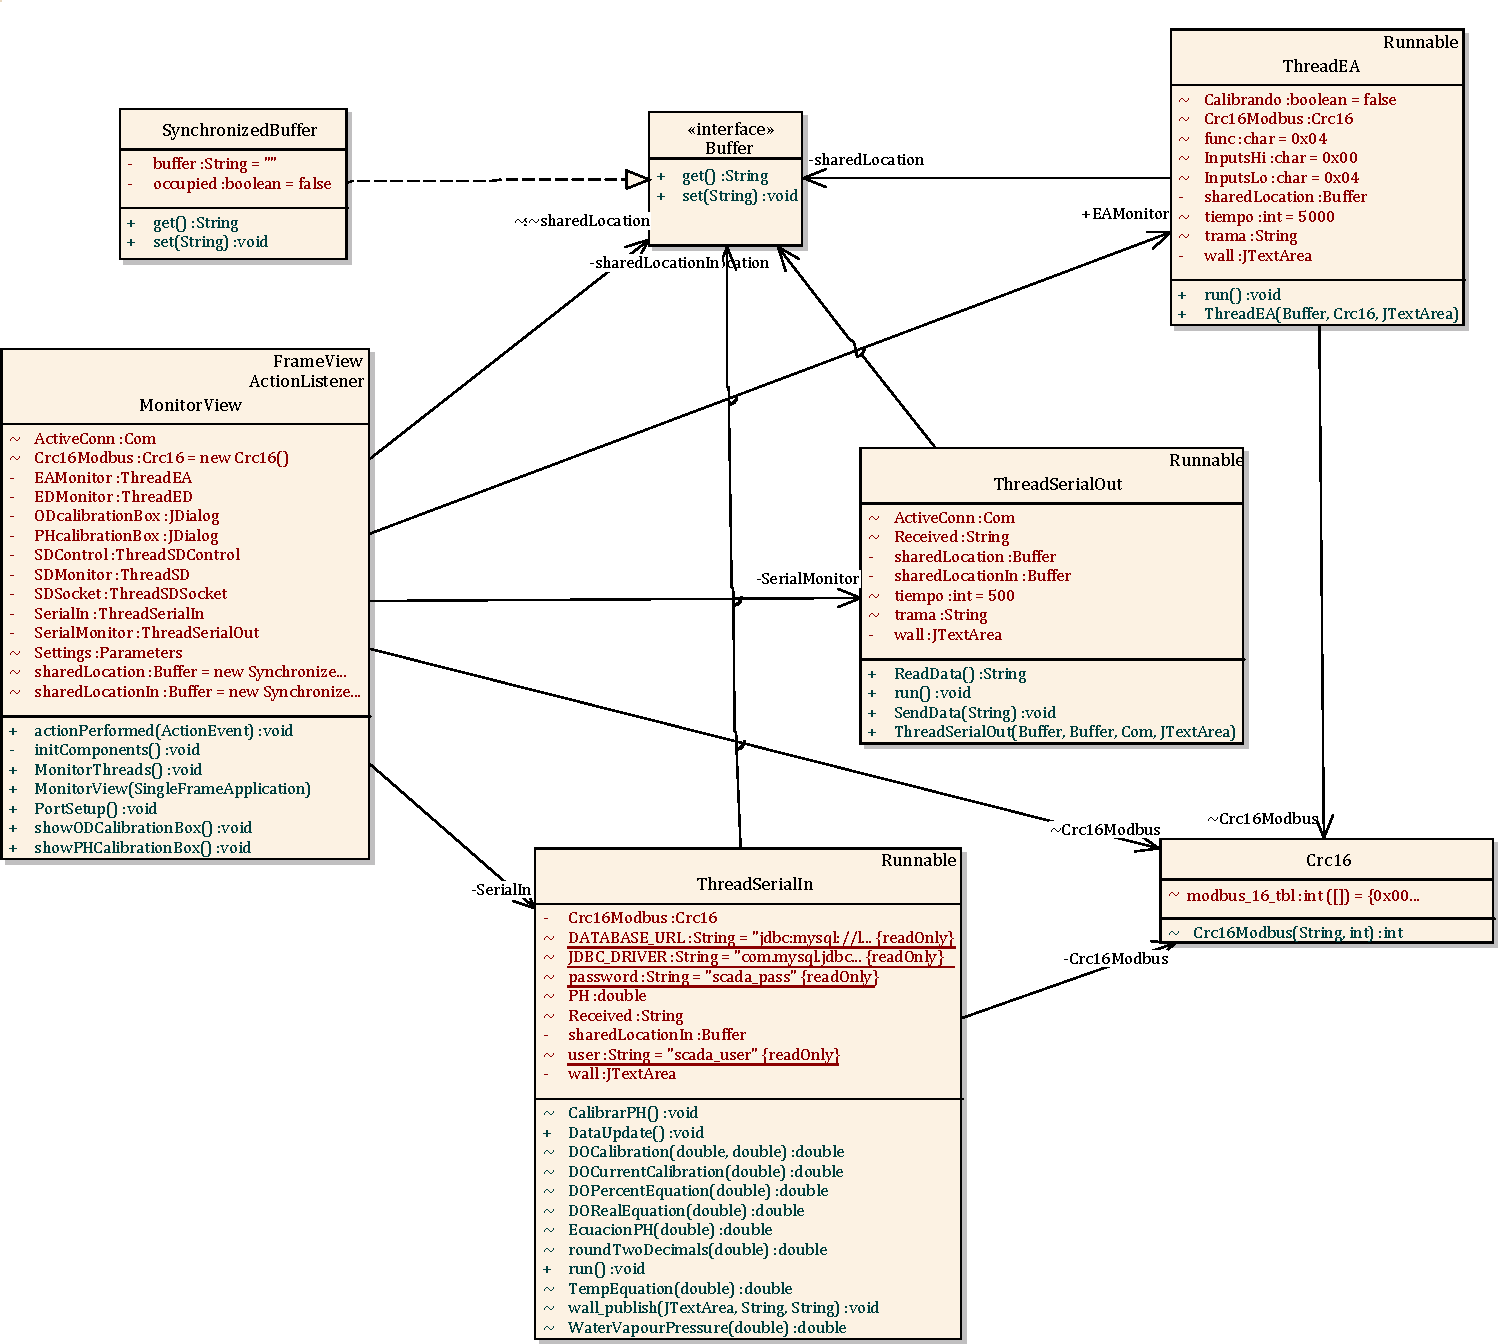
\includegraphics[scale=0.65]{Imagenes/Desarrollo/Dise�oSW/MTUClassEA.pdf}
\end{center}
 \caption{Diagrama de clases para monitoreo de entradas anal�gicas.} \label{fig:ap:MTUClassEA}
\end{figure}

\begin{figure}[H]
\begin{center}
 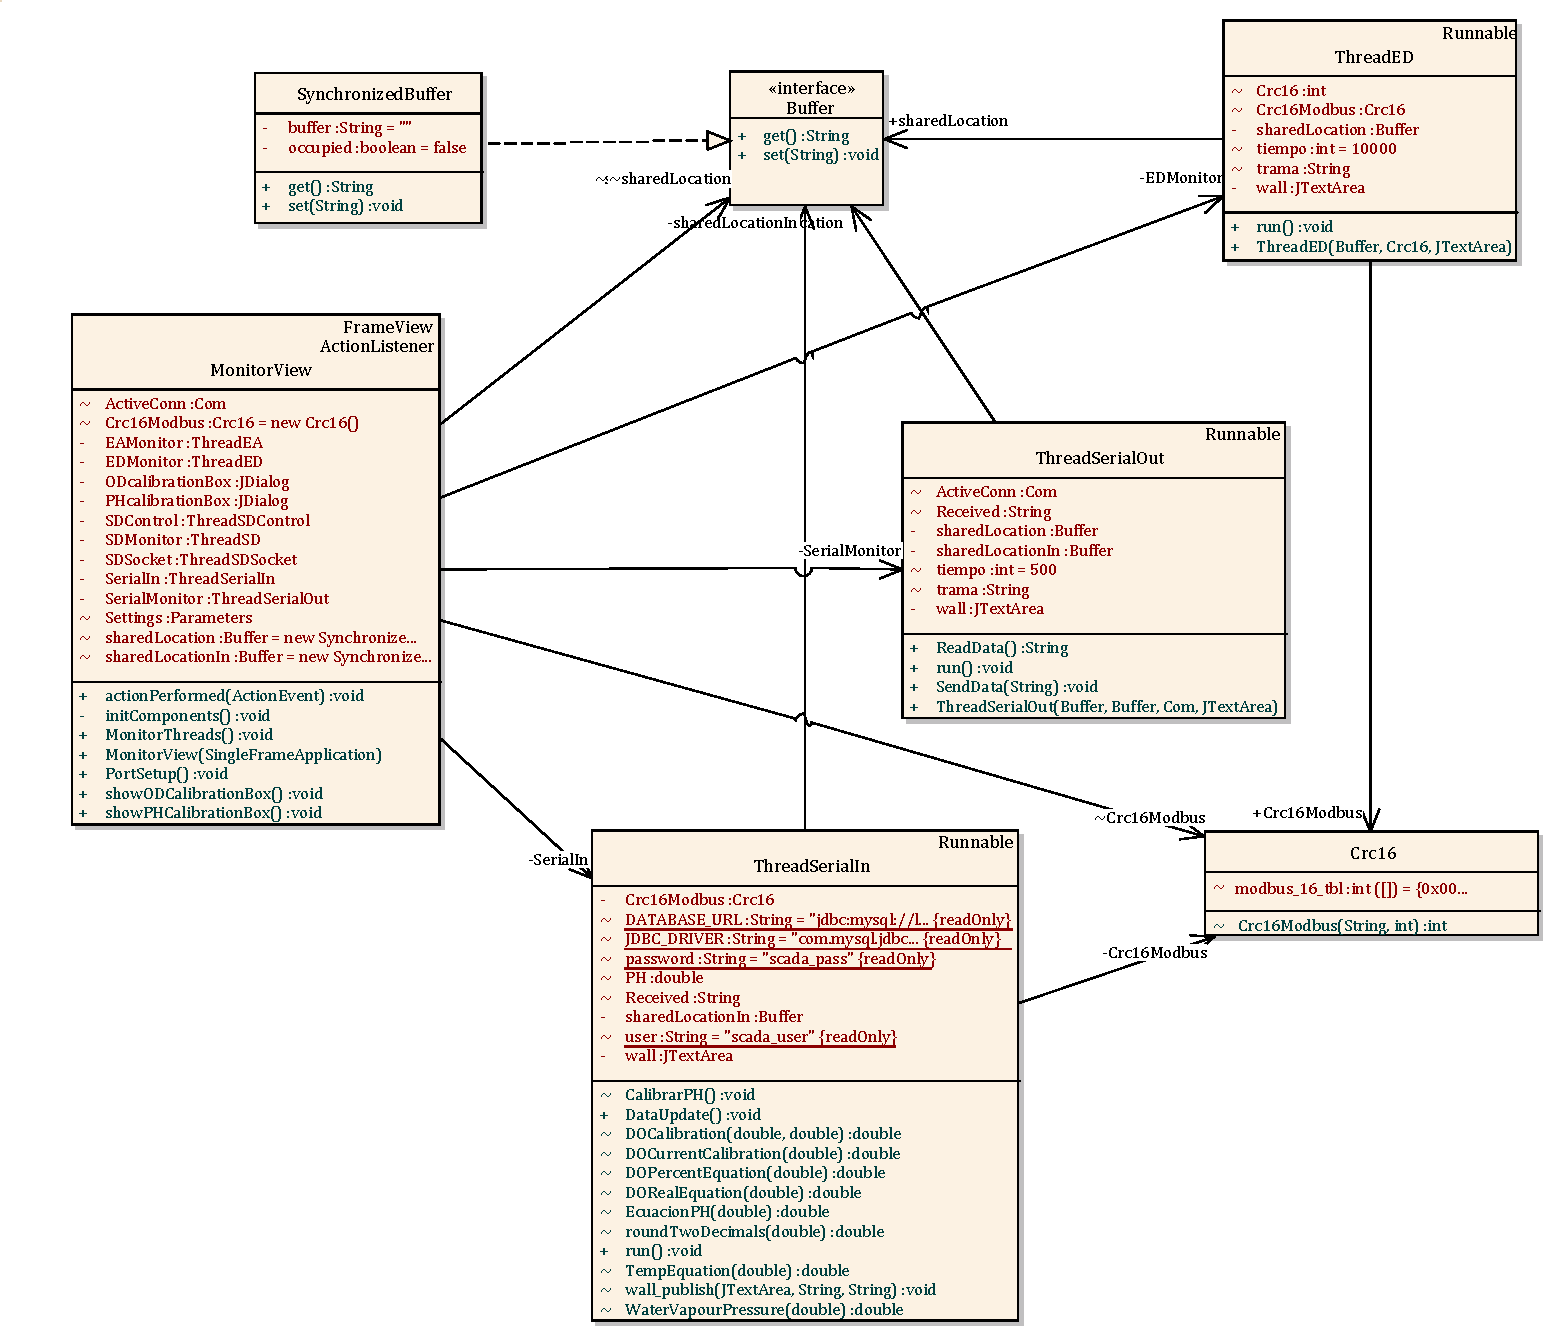
\includegraphics[scale=0.65]{Imagenes/Desarrollo/Dise�oSW/MTUClassED.pdf}
\end{center}
 \caption{Diagrama de clases para monitoreo de entradas digitales.} \label{fig:ap:MTUClassED}
\end{figure}

\begin{figure}[H]
\begin{center}
 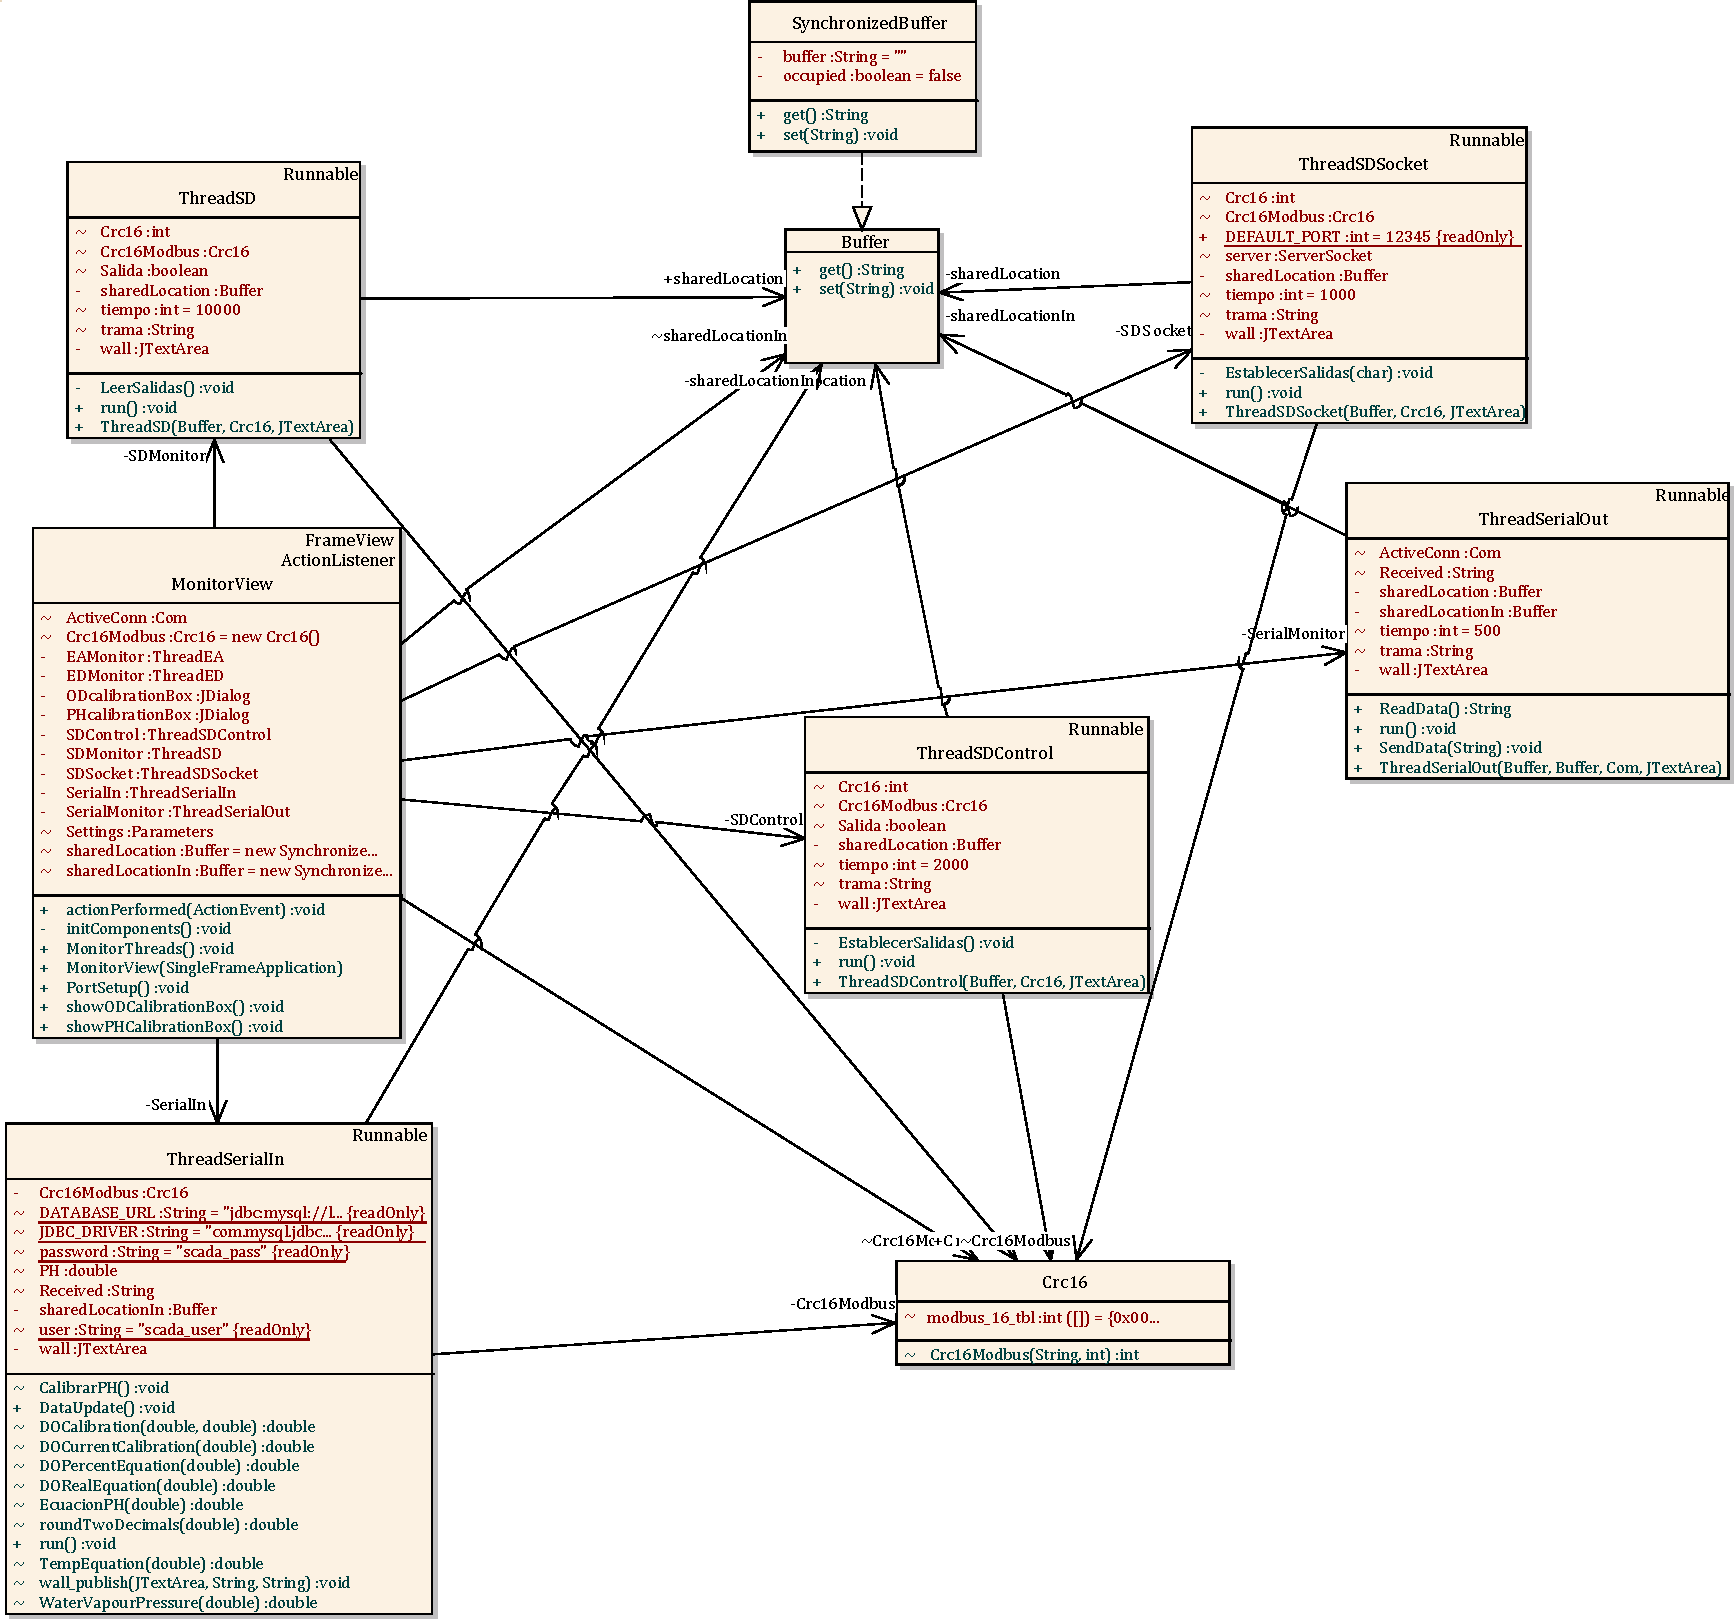
\includegraphics[scale=0.6]{Imagenes/Desarrollo/Dise�oSW/MTUClassSD.pdf}
\end{center}
 \caption{Diagrama de clases para monitoreo y control de salidas digitales.} \label{fig:ap:MTUClassSD}
\end{figure}

\begin{figure}[H]
\begin{center}
 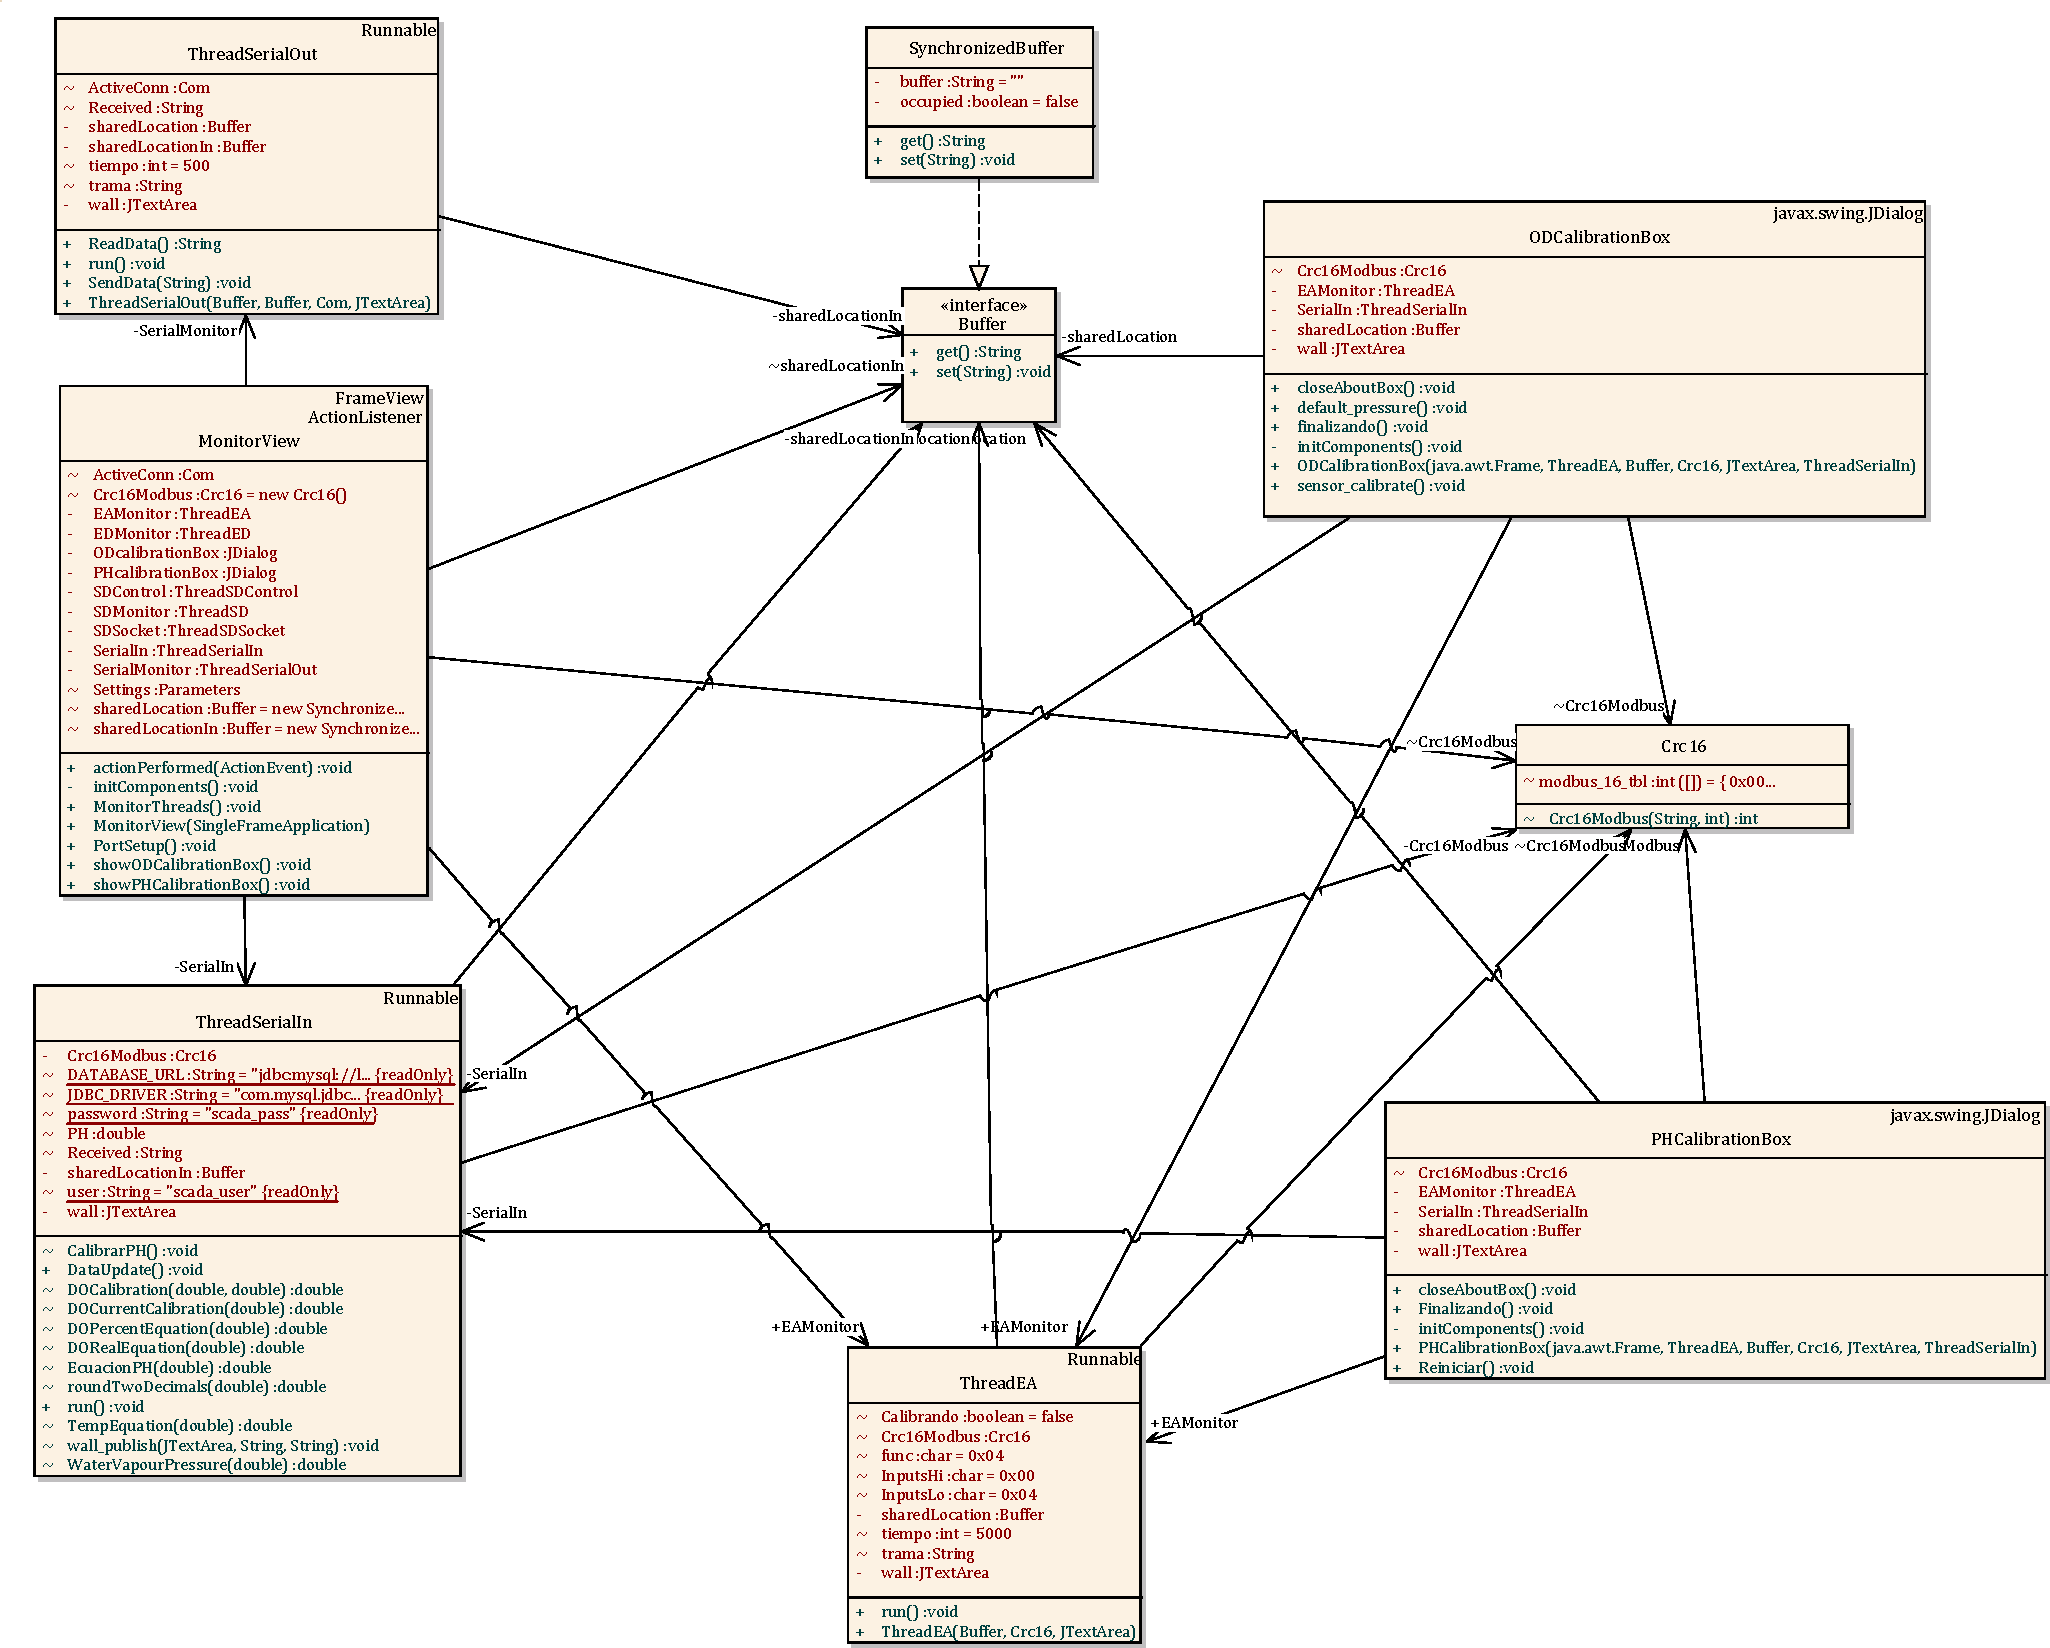
\includegraphics[scale=0.53]{Imagenes/Desarrollo/Dise�oSW/MTUClassCalibracion.pdf}
\end{center}
 \caption{Diagrama de clases para calibraci�n de sensores.} \label{fig:ap:MTUClassCalibracion}
\end{figure}

\newpage
\section{Diagramas de actividades}
\label{ap:SWMTU:Activity}

%En este ap�ndice se muestran los diagramas de actividades correspondientes a la gesti�n de la interfaz serial (Figura~\ref{fig:ap:MTUPuertoSerial}), procesamiento de ADUs de respuesta (Figura~\ref{fig:ap:MTUADUProcess}), establecer tiempo de muestreo (Figura~\ref{fig:ap:MTUTiempoMuestreo}), calibraci�n del sensor de pH y calibraci�n del sensor de OD (Figuras~\ref{fig:ap:MTUCalibracionpH} y~\ref{fig:ap:MTUCalibracionOD}).

\begin{figure}[H]
\begin{center}
 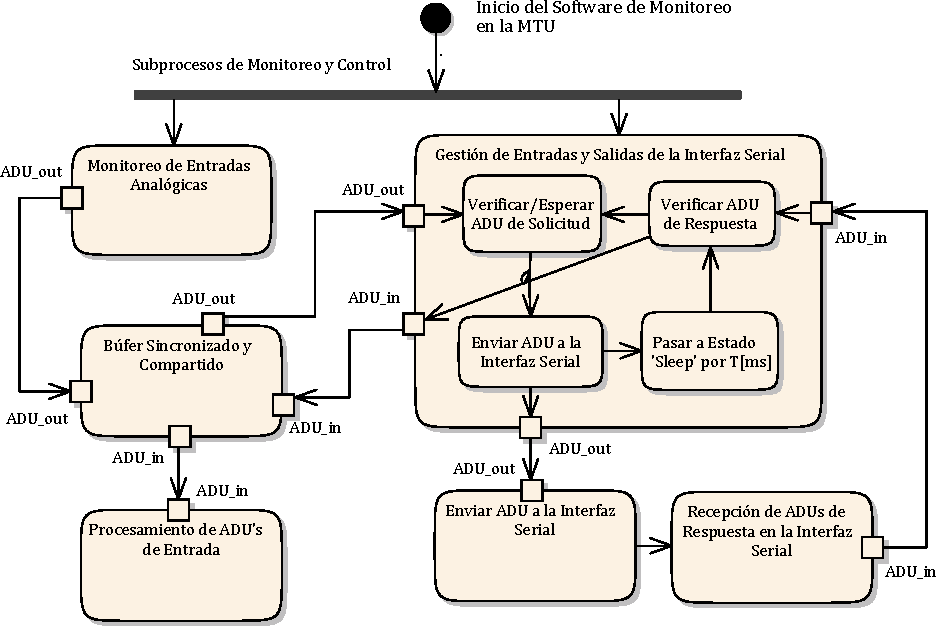
\includegraphics[scale=0.70]{Imagenes/Desarrollo/Dise�oSW/MTUPuertoSerial.pdf}
\end{center}
 \caption{Diagrama de actividades de la gesti�n de la interfaz serial.} \label{fig:ap:MTUPuertoSerial}
\end{figure}

\begin{figure}[H]
\begin{center}
 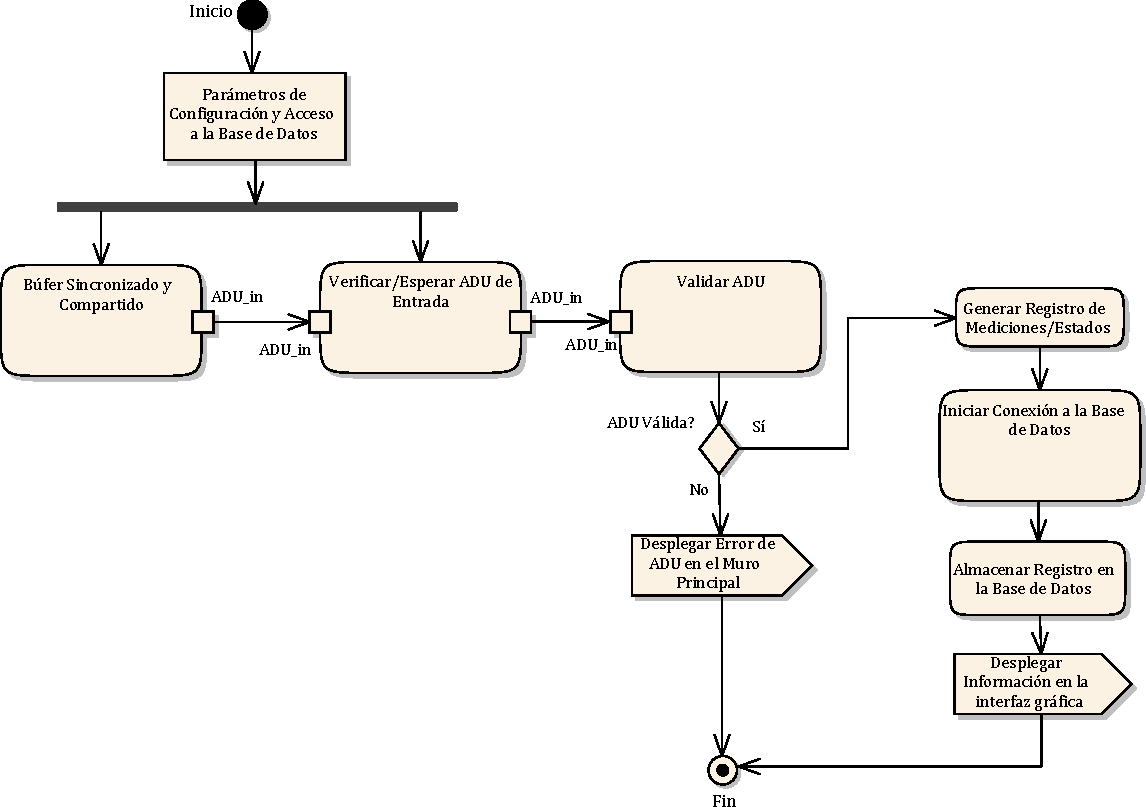
\includegraphics[scale=0.70]{Imagenes/Desarrollo/Dise�oSW/MTUADUProcess.pdf}
\end{center}
 \caption{Diagrama de actividades del procesamiento de ADUs.} \label{fig:ap:MTUADUProcess}
\end{figure}

\begin{figure}[H]
\begin{center}
 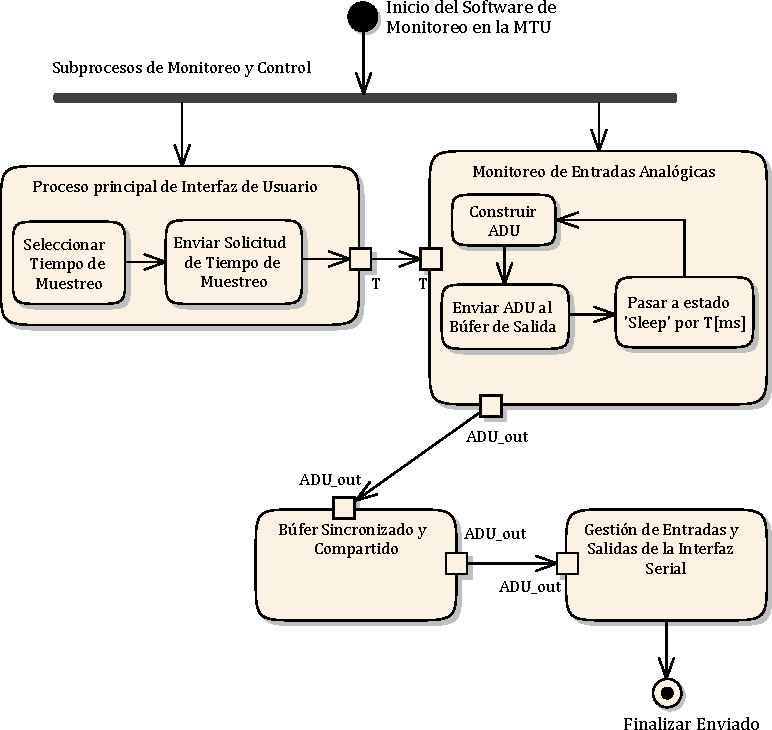
\includegraphics[scale=0.73]{Imagenes/Desarrollo/Dise�oSW/MTUTiempoMuestreo.pdf}
\end{center}
 \caption{Diagrama de actividades para establecer el tiempo de muestreo.} \label{fig:ap:MTUTiempoMuestreo}
\end{figure}

\begin{figure}[H]
\begin{center}
 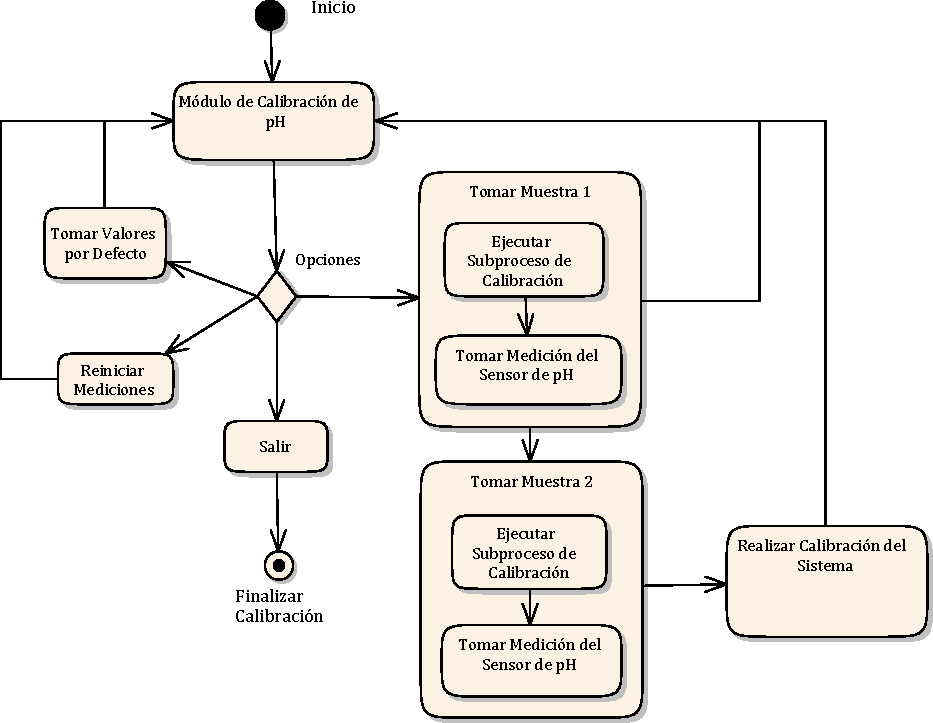
\includegraphics[scale=0.73]{Imagenes/Desarrollo/Dise�oSW/MTUCalibracionpH.pdf}
\end{center}
 \caption{Diagrama de actividades para calibrar el sensor de pH.} \label{fig:ap:MTUCalibracionpH}
\end{figure}

\begin{figure}[H]
\begin{center}
 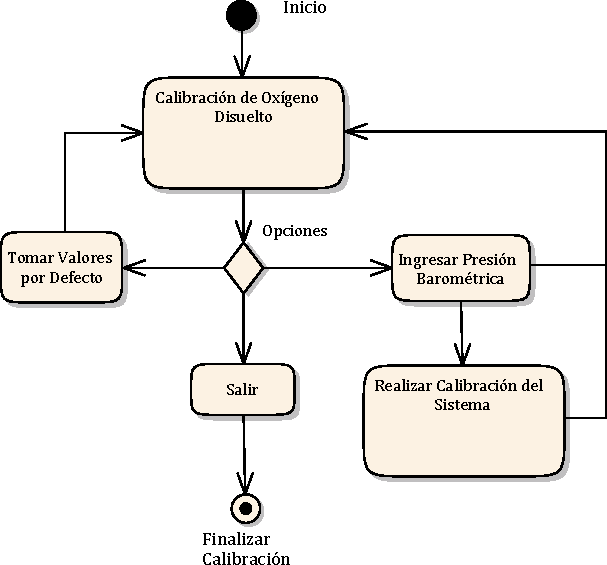
\includegraphics[scale=0.73]{Imagenes/Desarrollo/Dise�oSW/MTUCalibracionOD.pdf}
\end{center}
 \caption{Diagrama de actividades para calibrar el sensor de OD.} \label{fig:ap:MTUCalibracionOD}
\end{figure}